\chapter{Introdução} \label{Introducao}



Dentro deste universo, a engenharia de componentes é fundamental. Conforme os princípios de Projeto de Máquinas detalhados por \textcite{Norton2013}, todo sistema mecânico deve ser analisado sob a ótica de suas cargas, tensões e modos de falha potenciais. Um acessório de içamento, como a manilha, embora aparentemente simples, é um componente submetido a complexos estados de tensão. Fenômenos como a concentração de tensão em seus raios de curvatura e furos, e o risco de falha por fadiga após ciclos repetidos de carregamento, são fatores críticos que governam sua vida útil e segurança. \textcite{Norton2013} enfatiza que a aplicação de adequados fatores de segurança no projeto não é uma mera formalidade, mas uma necessidade para mitigar os riscos associados a incertezas nas cargas e nas propriedades do material. Ignorar esses princípios de engenharia na seleção ou no uso de uma manilha é negligenciar a base científica que garante a segurança da operação.

\begin{figure}[!htb]
   \centering
    \caption{Variedade de montagens para içamento e movimentação de cargas.}
    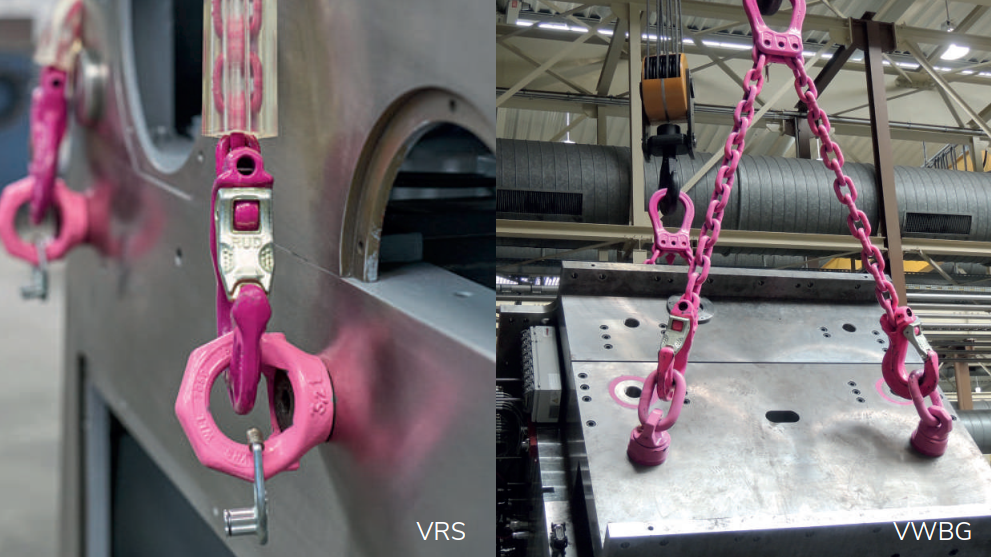
\includegraphics[width=1.0\linewidth]{Figuras/icamentoexemplos.png}\\    \hspace{1.5cm}\raggedright \fontsize{10}{12}\selectfont{Fonte: \textcite{RUD}.}
    \label{rudexemplos}
\end{figure}

A complexidade da seleção se aprofunda ao se consultar o portfólio de fabricantes especializados. O catálogo da \textcite{Crosby}, bem como a  \ref{rudexemplos}, que mostra montagens possíveis com produtos da RUD, referências no setor, ilustram que não existe uma solução única. A escolha deve ser criteriosa, distinguindo, por exemplo, entre manilhas tipo âncora (bow shackles), que são mais adequadas para cargas que vêm de múltiplos ângulos, e manilhas tipo reta (dee shackles), ideais para içamentos em linha. Adicionalmente, a seleção do sistema de travamento do pino é crucial: os modelos com pino roscado (screw pin) são práticos para montagens temporárias, enquanto os modelos com pino, porca e contrapino (bolt, nut, and cotter pin) são mandatórios para instalações de longo prazo ou onde há risco de vibração que poderia soltar o pino.



\section{Justificativa}

A utilização da análise de elementos finitos é uma excelente ferramenta para .

\section{Objetivos}

\subsection{Objetivo geral}

O objetivo deste trabalho é .  


\subsection{Objetivos específicos}
\begin{enumerate}

    \item Otimizar a .

    \item Definir .

    \item Definir .
    
\end{enumerate}